%%%%%%%%%%%%%%
%% Run LaTeX on this file several times to get Table of Contents,
%% cross-references, and citations.

%% If you have font problems, you may edit the w-bookps.sty file
%% to customize the font names to match those on your system.

%% w-bksamp.tex. Current Version: Feb 16, 2012
%%%%%%%%%%%%%%%%%%%%%%%%%%%%%%%%%%%%%%%%%%%%%%%%%%%%%%%%%%%%%%%%
%
%  Sample file for
%  Wiley Book Style, Design No.: SD 001B, 7x10
%  Wiley Book Style, Design No.: SD 004B, 6x9
%
%
%  Prepared by Amy Hendrickson, TeXnology Inc.
%  http://www.texnology.com
%%%%%%%%%%%%%%%%%%%%%%%%%%%%%%%%%%%%%%%%%%%%%%%%%%%%%%%%%%%%%%%%

%%%%%%%%%%%%%
% 7x10
%\documentclass{wileySev}

% 6x9
\documentclass{wileySix}

\usepackage{graphicx}
\usepackage{listings}

\usepackage{color}
 
\definecolor{codegreen}{rgb}{0,0.6,0}
\definecolor{codegray}{rgb}{0.5,0.5,0.5}
\definecolor{codepurple}{rgb}{0.58,0,0.82}
\definecolor{backcolour}{rgb}{0.95,0.95,0.92}
 
\lstdefinestyle{mystyle}{
    backgroundcolor=\color{backcolour},   
    commentstyle=\color{codegreen},
    keywordstyle=\color{magenta},
    numberstyle=\tiny\color{codegray},
    stringstyle=\color{codepurple},
    basicstyle=\footnotesize,
    breakatwhitespace=false,         
    breaklines=true,                 
    captionpos=b,                    
    keepspaces=true,                 
    numbers=left,                    
    numbersep=5pt,                  
    showspaces=false,                
    showstringspaces=false,
    showtabs=false,                  
    tabsize=2,
    language=sh
}
 
\lstset{style=mystyle}

%%%%%%%
%% for times math: However, this package disables bold math (!)
%% \mathbf{x} will still work, but you will not have bold math
%% in section heads or chapter titles. If you don't use math
%% in those environments, mathptmx might be a good choice.

% \usepackage{mathptmx}

% For PostScript text
\usepackage{w-bookps}

%%%%%%%%%%%%%%%%%%%%%%%%%%%%%%%%%%%%%%%%%%%%%%%%%%%%%%%%%%%%%%%%
%% Other packages you might want to use:

% for chapter bibliography made with BibTeX
% \usepackage{chapterbib}

% for multiple indices
% \usepackage{multind}

% for answers to problems
% \usepackage{answers}

%%%%%%%%%%%%%%%%%%%%%%%%%%%%%%
%% Change options here if you want:
%%
%% How many levels of section head would you like numbered?
%% 0= no section numbers, 1= section, 2= subsection, 3= subsubsection
%%==>>
\setcounter{secnumdepth}{3}

%% How many levels of section head would you like to appear in the
%% Table of Contents?
%% 0= chapter titles, 1= section titles, 2= subsection titles, 
%% 3= subsubsection titles.
%%==>>
\setcounter{tocdepth}{2}

%% Cropmarks? good for final page makeup
%% \docropmarks

%%%%%%%%%%%%%%%%%%%%%%%%%%%%%%
%
% DRAFT
%
% Uncomment to get double spacing between lines, current date and time
% printed at bottom of page.
% \draft
% (If you want to keep tables from becoming double spaced also uncomment
% this):
% \renewcommand{\arraystretch}{0.6}
%%%%%%%%%%%%%%%%%%%%%%%%%%%%%%

%%%%%%% Demo of section head containing sample macro:
%% To get a macro to expand correctly in a section head, with upper and
%% lower case math, put the definition and set the box 
%% before \begin{document}, so that when it appears in the 
%% table of contents it will also work:

\newcommand{\VT}[1]{\ensuremath{{V_{T#1}}}}

%% use a box to expand the macro before we put it into the section head:

\newbox\sectsavebox
\setbox\sectsavebox=\hbox{\boldmath\VT{xyz}}

%%%%%%%%%%%%%%%%% End Demo


\begin{document}


\booktitle{Cerdas Menguasai Git}
\subtitle{Dalam 24 Jam}

\authors{Rolly M. Awangga\\
\affil{Informatics Research Center}
%Floyd J. Fowler, Jr.\\
%\affil{University of New Mexico}
}

\offprintinfo{Cerdas Menguasai Git, First Edition}{Rolly M. Awangga}

%% Can use \\ if title, and edition are too wide, ie,
%% \offprintinfo{Survey Methodology,\\ Second Edition}{Robert M. Groves}

%%%%%%%%%%%%%%%%%%%%%%%%%%%%%%
%% 
\halftitlepage

\titlepage


\begin{copyrightpage}{2019}
%Survey Methodology / Robert M. Groves . . . [et al.].
%\       p. cm.---(Wiley series in survey methodology)
%\    ``Wiley-Interscience."
%\    Includes bibliographical references and index.
%\    ISBN 0-471-48348-6 (pbk.)
%\    1. Surveys---Methodology.  2. Social 
%\  sciences---Research---Statistical methods.  I. Groves, Robert M.  II. %
%Series.\\
%
%HA31.2.S873 2007
%001.4'33---dc22                                             2004044064
\end{copyrightpage}

\dedication{`Jika Kamu tidak dapat menahan lelahnya belajar, 
Maka kamu harus sanggup menahan perihnya Kebodohan.'
~Imam Syafi'i~}

\begin{contributors}
\name{Rolly Maulana Awangga,} Informatics Research Center., Politeknik Pos Indonesia, Bandung,
Indonesia



\end{contributors}

\contentsinbrief
\tableofcontents
\listoffigures
\listoftables
\lstlistoflistings


\begin{foreword}
Sepatah kata dari Kaprodi, Kabag Kemahasiswaan dan Mahasiswa
\end{foreword}

\begin{preface}
Buku ini diciptakan bagi yang awam dengan flask sekalipun.

\prefaceauthor{R. M. Awangga}
\where{Bandung, Jawa Barat\\
Februari, 2019}
\end{preface}


\begin{acknowledgments}
Terima kasih atas semua masukan dari para mahasiswa agar bisa membuat buku ini 
lebih baik dan lebih mudah dimengerti.

Terima kasih ini juga ditujukan khusus untuk team IRC yang 
telah fokus untuk belajar dan memahami bagaimana buku ini mendampingi proses 
Intership.
\authorinitials{R. M. A.}
\end{acknowledgments}

\begin{acronyms}
\acro{ACGIH}{American Conference of Governmental Industrial Hygienists}
\acro{AEC}{Atomic Energy Commission}
\acro{OSHA}{Occupational Health and Safety Commission}
\acro{SAMA}{Scientific Apparatus Makers Association}
\end{acronyms}

\begin{glossary}
\term{git}Merupakan manajemen sumber kode yang dibuat oleh linus torvald.

\term{bash}Merupakan bahasa sistem operasi berbasiskan *NIX.

\term{linux}Sistem operasi berbasis sumber kode terbuka yang dibuat oleh Linus Torvald
\end{glossary}

\begin{symbols}
\term{A}Amplitude

\term{\hbox{\&}}Propositional logic symbol 

\term{a}Filter Coefficient

\bigskip

\term{\mathcal{B}}Number of Beats
\end{symbols}

\begin{introduction}

%% optional, but if you want to list author:

\introauthor{Rolly Maulana Awangga, S.T., M.T.}
{Informatics Research Center\\
Bandung, Jawa Barat, Indonesia}

Pada era disruptif  \index{disruptif}\index{disruptif!modern} 
saat ini. git merupakan sebuah kebutuhan dalam sebuah organisasi pengembangan perangkat lunak.
Buku ini diharapkan bisa menjadi penghantar para programmer, analis, IT Operation dan Project Manajer.
Dalam melakukan implementasi git pada diri dan organisasinya.

Rumusnya cuman sebagai contoh aja biar keren\cite{awangga2018sampeu}.

\begin{equation}
ABC {\cal DEF} \alpha\beta\Gamma\Delta\sum^{abc}_{def}
\end{equation}

\end{introduction}

%%%%%%%%%%%%%%%%%%Isi Buku_

\chapter{Judul Bagian Pertama}
\section{Perintah Navigasi}
Perintah navigasi direktori


\chapter{Judul Bagian Kedua}
\section{Variabel Python}
Variabel merupakan sebuah ruang kosong untuk menyimapan suatu nilai atau data. Pada saat anda membuat sebuah variabel berarti anda sedang memesan sebuah ruang kosong di memori. Isi dari variabel itu dapat berubah atau mutable sesuai dengan operasi yang diinginkan. Saat program dieksekusi maka variabellah yang bertugas menyimpan data. 

Variabel dapat menyimpan berbagai macam tipe data. Dalam pemrograman Python, variabel mempunyai sifat dinamis, yang berarti variabel Python tidak perlu ditentukan tipe data tertentu dan variabel pada Python dapat diubah saat program dieksekusi.

Peraturan penulisan variable Python :
\begin{enumerate}
\item Karakter pertama harus berupa huruf atau garis bawah atau underscore (\_)
\item Karakter selanjutnya dapat berupa huruf, garis bawah/underscore (\_) atau angka
\item Karakter pada nama variabel bersifat sensitif (case-sensitif). Artinya penggunaan uruf besar dan huruf keci sangat berpengaruh. Sebagai contoh, variabel Mahasiswa dan mahasiswa adalah variabel yang berbeda.
\item Nama variabel tidak boleh menggunakan kata kunci yang sudah ada pada Python.
\end{enumerate}
Untuk membuat variabel Python caraya sangat mudah, cukup buat nama vairabel lalu diikiikuti oleh = dan mengisinya dengan nilai yang dinginkan.

\subsection{Contoh Pembuatan Variabel Python}
Misalnya ada variabel “nama” dengan nilai “Poltekpos”. Maka penulisan variabelnya seperti pada gambar \ref{fig:penulisanvariabel}:
\begin{figure}[!htbp]
	\centerline{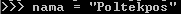
\includegraphics[width=0.45\textwidth]{figures/2/penulisanvariabel.PNG}}
	\caption{Penulisan Variabel}
	\label{fig:penulisanvariabel}
\end{figure}

Kemudian perintahkan print untuk menampilkan isi dari variabel. Caranya: \verb|Print namavariabel|
Contohnya seperti pada gambar \ref{fig:hasilperintahprint} :
\begin{figure}[!htbp]
	\centerline{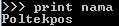
\includegraphics[width=0.55\textwidth]{figures/2/hasilperintahprint}}
	\caption{Hasil Perintah Print}
	\label{fig:hasilperintahprint}
\end{figure}

\subsection{Menghapus Variabel}
Untuk menghapus variabel caranya sangat mudah. Anda cukup menggunakan perintah del() untuk menghapus variabel yang sudah tidak dibutuhkan lagi. Perintah delete, \verb|del(namavariabel)|
Contohnya seperti pada gambar \ref{fig:perintahdel} :
\begin{figure}[!htbp]
	\centerline{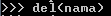
\includegraphics[width=0.40\textwidth]{figures/2/perintahdel.PNG}}
	\caption{Perintah del}
	\label{fig:perintahdel}
\end{figure}

Untuk mengecek apakah variabelnya berhasil dihapus anda bisa menggunakan perintah print seperti pada gambar \ref{fig:perintahprint}. 
\begin{figure}[!htbp]
	\centerline{
\includegraphics[width=0.55\textwidth]{figures/2/perintahprint.PNG}}
	\caption{Perintah Print}
	\label{fig:perintahprint}
\end{figure}

Jika hasilnya seperti gambar \ref{fig:afterdelete} maka variabel telah berhasil dihapus.
\begin{figure}[!htbp]
	\centerline{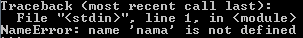
\includegraphics[width=0.75\textwidth]{figures/2/afterdelete.PNG}}
	\caption{Hasil perintah print setelah variabel di delete}
	\label{fig:afterdelete}
\end{figure}

\section{Input Output User}
Input adalah masukan yang anda berikan kepada sebuah program dan system akan memproses lalu menampilkan ouputnya.

\subsection{Cara mengambil input pada keyboard}
Di dalam python sudah terdapat fungsi input() dan raw\_input(). input() digunakan untuk masukan bernilai angka sedangkan raw\_input untuk masukan bernilai teks.

Cara penggunaannya seperti ini \verb|nama\_variabel = input(“masukkan teks”)|

Teks yang anda masukkan akan disimpan ke nama\_variabel.

Contohnya seperti pada listing \ref{lst:iouser} :
\lstinputlisting[caption=Contoh kode input output, label={lst:iouser}]{src/2/iouser.py}

Hasilnya seperti pada gambar \ref{fig:hasilinput}:
\begin{figure}[!htbp]
	\centerline{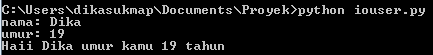
\includegraphics[width=0.85\textwidth]{figures/2/hasilinput.PNG}}
	\caption{Hasil input}
	\label{fig:hasilinput}
\end{figure}

\subsection{Menampilkan Variabel dan Teks}
Anda bisa menampilkan variabel dan teks menggunakan perintah print seperti pada listing \ref{lst:halo}
\lstinputlisting[caption=Perintah menampilkan variabel dan teks, label={lst:halo}]{src/2/halo.py}

Hasilnya seperti pada gambar \ref{fig:showvar}:
\begin{figure}[!htbp]
	\centerline{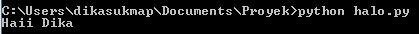
\includegraphics[width=0.85\textwidth]{figures/2/showvar.PNG}}
	\caption{Hasil menampilkan variabel dan teks}
	\label{fig:showvar}
\end{figure}

Tanda koma pada kode diatas merupakan sebuah spasi apabila kode dieksekusi.

\section{Operator Dasar}
Operator python adalah simbol yang melakukan operasi pada satu atau lebih operan. Operan adalah variabel atau nilai yang digunakan untuk melakukan operasi.
Operator pada Python dibagi menjadi beberapa jenis, yaitu :

\subsection{Operator Aritmatika}
% Please add the following required packages to your document preamble:
% \usepackage{graphicx}
\begin{table}[]
\caption{Operator Aritmatika}
\label{tab:my-table}
\resizebox{\textwidth}{!}{%
\begin{tabular}{|l|l|l|}
\hline
Operator           & Contoh      & Keterangan                                                                                                 \\ \hline
Penjumlahan +      & 3 + 1 = 4   & Menjumlahkan masing - masing bilangan                                                                      \\ \hline
Pengurangan -      & 4 - 1 = 3   & Mengurangi nilai operan di sebelah kiri menggunakan operan di sebelah kanan                                \\ \hline
Perkalian *        & 2 * 1 = 2   & Mengalikan dua bilangan                                                                                    \\ \hline
Pembagian /        & 4 / 2 = 2   & Untuk membagi operan di sebelah kiri menggunakan operan di sebelah kanan                                   \\ \hline
Sisa Bagi \%       & 13 \% 4 = 1 & Mendapatkan sisa pembagian dari operan di sebelah kiri operator ketika dibagi oleh operan di sebelah kanan \\ \hline
Pangkat **         & 6 ** 2 = 36 & Memangkatkan operan disebelah kiri operator dengan operan di sebelah kanan operator                        \\ \hline
Pembagian Bulat // & 10 // 3 = 3 & Sama seperti pembagian. Hanya saja angka dibelakang koma dihilangkan                                       \\ \hline
\end{tabular}%
}
\end{table}

Contoh penggunaannya seperti pada listing \ref{lst:aritmatika} :
\lstinputlisting[caption=Contoh operator aritmatika, label={lst:aritmatika}]{src/2/operator_aritmatika.py}

Hasilnya seperti pada gambar \ref{fig:aritmatika}:
\begin{figure}[!htbp]
	\centerline{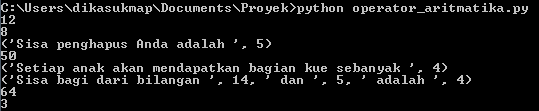
\includegraphics[width=0.85\textwidth]{figures/2/aritmatika.PNG}}
	\caption{Hasil contoh operator aritmatika}
	\label{fig:aritmatika}
\end{figure}

\subsection{Operator Perbandingan}
% Please add the following required packages to your document preamble:
% \usepackage{graphicx}
\begin{table}[]
\caption{Operator Perbandingan}
\label{tab:my-table}
\resizebox{\textwidth}{!}{%
\begin{tabular}{lll}
Operator                                    & Contoh                      & Keterangan                                                                                                       \\
Sama dengan =                               & 2 == 2                      & bernilai True Jika masing-masing operan memiliki nilai yang sama, maka kondisi bernilai benar atau True.         \\
Tidak sama dengan !=                        & 2 != 2                      & bernilai False Akan menghasilkan nilai kebalikan dari kondisi sebenarnya.                                        \\
Tidak sama dengan \textless{}\textgreater{} & 2 \textless{}\textgreater 2 & bernilai False Akan menghasilkan nilai kebalikan dari kondisi sebenarnya                                         \\
Lebih besar dari \textgreater{}             & 3 \textgreater 2            & bernilai True Jika nilai operan kiri lebih besar dari nilai operan kanan, maka kondisi menjadi benar.            \\
Lebih kecil dari \textless{}                & 2 \textless 3               & bernilai True Jika nilai operan kiri lebih kecil dari nilai operan kanan, maka kondisi menjadi benar.            \\
Lebih besar / sama dengan \textgreater{}=   & 3 \textgreater{}= 2         & bernilai True Jika nilai operan kiri lebih besar dari nilai operan kanan, atau sama, maka kondisi menjadi benar. \\
Lebih kecil / sama dengan =                 & 2 \textless{}= 3            & bernilai True Jika nilai operan kiri lebih kecil dari nilai operan kanan, atau sama, maka kondisi menjadi benar.
\end{tabular}%
}
\end{table}

Contoh penggunaannya seperti pada listing \ref{lst:perbandingan} :
\lstinputlisting[caption=Contoh operator perbandingan, label={lst:perbandingan}]{src/2/operator_perbandingan.py}

Hasilnya seperti pada gambar \ref{fig:perbandingan}:
\begin{figure}[!htbp]
	\centerline{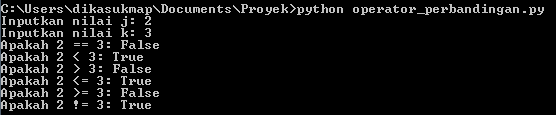
\includegraphics[width=0.85\textwidth]{figures/2/perbandingan.PNG}}
	\caption{Hasil contoh operator perbandingan}
	\label{fig:perbandingan}
\end{figure}

\subsection{Operator Penugasan}
Operator Penugasan digunakan untuk memodifikasi sebuah nilai yang ada pada variabel tertentu.
% Please add the following required packages to your document preamble:
% \usepackage{graphicx}
\begin{table}[]
\caption{Operator Penugasan}
\label{tab:my-table}
\resizebox{\textwidth}{!}{%
\begin{tabular}{lll}
Operator                        & Contoh  & Penjelasan                                                                                                                                   \\
Sama dengan =                   & A = 3   & Memberikan nilai di kanan ke dalam variabel yang berada di sebelah kiri.                                                                     \\
Tambah sama dengan +=           & A += 3  & Memberikan nilai variabel dengan nilai variabel itu sendiri ditambah dengan nilai di sebelah kanan.                                          \\
Kurang sama dengan -=           & A -= 3  & Memberikan nilai variabel dengan nilai variabel itu sendiri dikurangi dengan nilai di sebelah kanan.                                         \\
Kali sama dengan *=             & A *= 3  & Memberikan nilai variabel dengan nilai variabel itu sendiri dikali dengan nilai di sebelah kanan.                                            \\
Bagi sama dengan /=             & A /= 6  & Memberikan nilai variabel dengan nilai variabel itu sendiri dibagi dengan nilai di sebelah kanan.                                            \\
Sisa bagi sama dengan  \%=      & A \%= 3 & Memberikan nilai variabel dengan nilai variabel itu sendiri dibagi dengan nilai di sebelah kanan. Yang diambil nantinya adalah sisa baginya. \\
Pangkat sama dengan **=         & A **= 2 & Memberikan nilai variabel dengan nilai variabel itu sendiri dipangkatkan dengan nilai di sebelah kanan.                                      \\
Pembagian bulat sama dengan //= & A //= 4 & Membagi bulat operan sebelah kiri operator dengan operan sebelah kanan operator kemudian hasilnya diisikan ke operan sebelah kiri.          
\end{tabular}%
}
\end{table}

Contoh penggunaannya seperti pada listing \ref{lst:penugasan} :
\lstinputlisting[caption=Contoh operator penugasan, label={lst:penugasan}]{src/2/operator_penugasan.py}

Hasilnya seperti pada gambar \ref{fig:penugasan}:
\begin{figure}[!htbp]
	\centerline{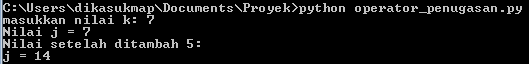
\includegraphics[width=0.85\textwidth]{figures/2/penugasan.PNG}}
	\caption{Hasil contoh operator penugasan}
	\label{fig:penugasan}
\end{figure}

\subsection{Operator Logika}
Operator logika digunakan untuk membuat operasi logika, seperti logika AND, OR, dan NOT.

\begin{table}[]
\caption{Operator Logika}
\label{tab:my-table}
\begin{tabular}{|l|l|}
\hline
Nama             & Simbol \\ \hline
Logika And       & and    \\ \hline
Logika Or        & or     \\ \hline
Negasi/kebalikan & not    \\ \hline
\end{tabular}
\end{table}

Contoh penggunaannya seperti pada listing \ref{lst:logika} :
\lstinputlisting[caption=Contoh operator logika, label={lst:logika}]{src/2/operator_logika.py}

Hasilnya seperti pada gambar \ref{fig:logika}:
\begin{figure}[!htbp]
	\centerline{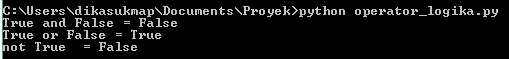
\includegraphics[width=0.85\textwidth]{figures/2/logika.PNG}}
	\caption{Hasil contoh operator logika}
	\label{fig:logika}
\end{figure}

\subsection{Operator Bitwise}
Operator bitwise digunakan untuk melakukan operasi dalam bentuk bit atau biner.

\begin{table}[]
\caption{Operator Bitwise}
\label{tab:my-table}
\begin{tabular}{|l|l|}
\hline
Nama        & Simbol                       \\ \hline
AND         & \&                           \\ \hline
OR          & |                            \\ \hline
XOR         & \textasciicircum{}           \\ \hline
Negasi      & $\sim$                       \\ \hline
Left Shift  & \textless{}\textless{}       \\ \hline
Right Shift & \textgreater{}\textgreater{} \\ \hline
\end{tabular}
\end{table}

Contoh penggunaannya seperti pada listing \ref{lst:bitwise} :
\lstinputlisting[caption=Contoh operator bitwise, label={lst:bitwise}]{src/2/operator_bitwise.py}

Hasilnya seperti pada gambar \ref{fig:bitwise}:
\begin{figure}[!htbp]
	\centerline{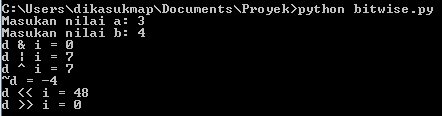
\includegraphics[width=0.85\textwidth]{figures/2/bitwise.PNG}}
	\caption{Hasil contoh operator bitwise}
	\label{fig:bitwise}
\end{figure}

\subsection{Prioritas Eksekusi Operator di Python}
Berikut adalah prioritas yang dieksekusi di dalam perintah python. Maksudnya adalah di dalam python terdapat beberapa operator dan prioritasnya masing - masing. Tabel \ref{tab:eksekusi} merupakan prioritas python dari mulai yang pertama sampai dengan yang terakhir dalam proses pengeksekusian :
\begin{table}[]
\caption{Prioritas Eksekusi Operator di Python}
\label{tab:my-table}
\begin{tabular}{|l|l|}
\hline
Operator                                                & Keterangan   \\ \hline
**                                                      & Aritmatika   \\ \hline
$\sim$,+,-                                              & Bitwise      \\ \hline
*,/,//,\%                                               & Arimatika    \\ \hline
+,-                                                     & Aritmatika   \\ \hline
\textgreater{}\textgreater{},\textless{}\textless{}     & Bitwise      \\ \hline
\&                                                      & Bitwise      \\ \hline
\textasciicircum{},|                                    & Bitwise      \\ \hline
\textless{}=,\textless{},\textgreater{},\textgreater{}= & Perbandingan \\ \hline
\textless{}\textgreater{},==,!=                         & Perbandingan \\ \hline
Err:509                                                 & Penugasan    \\ \hline
Is,is not                                               & Identitas    \\ \hline
In,not in                                               & Keanggotaan  \\ \hline
Not,or,and                                              & Logika       \\ \hline
\end{tabular}
\end{table}

\section{Perulangan / Loop}
Secara umum, perintah pada bahasa pemrograman Python akan dijalankan secara berurutan. Pernyataan pertama dalam sebuah fungsi dijalankan pertama, lalu diikuti oleh yang kedua, dan seterusnya. Tetapi akan ada situasi dimana Anda harus menulis banyak kode, dimana kode tersebut sangat banyak. Jika dilakukan secara manual maka Anda hanya akan membuang-buang waktu dan tenaga. Untuk itu Anda perlu menggunakan pengulangan atau loop di dalam bahasa pemrograman Python.

Di dalam bahasa pemrograman Python pengulangan dibagi menjadi 3 bagian, yaitu :
\subsection{While Loop}
Pada while loop pernyataan akan dieksekusi berkali-kali selama kondisi bernilai benar atau true.

Contoh penggunaannya seperti pada listing \ref{lst:whileloop} :
\lstinputlisting[caption=Koding while loop, label={lst:whileloop}]{src/2/whileloop.py}

\subsection{For Loop}
For Loop memiliki kemampuan untuk mengulangi item dari urutan apapun,misalnya string atau list.

Contoh penggunaannya seperti pada listing \ref{lst:forloop} :
\lstinputlisting[caption=Koding for loop, label={lst:forloop}]{src/2/forloop.py}
 
\subsection{Nested Loop} 
Nested loop memungkinkan terjadi sebuah pengulangan di dalam pengulangan lainnya.

Contoh penggunaannya seperti pada listing \ref{lst:nestedloop} :
\lstinputlisting[caption=Koding nested loop, label={lst:nestedloop}]{src/2/nestedloop.py}

\section{Kondisi}
\subsection{Kondisi IF}
Pada saat pengambilan keputusan (kondisi if) digunakan untuk mengantisipasi kondisi yang akan terjadi saat program dijalankan.Dan akan menentukan tindakan apa yang akan diambil sesuai dengan kondisi program pada saat dieksekusi.

Pada python ada beberapa kondisi diantaranya adalah if, else, dan elif. Kondisi if hanya bisa digunakan pada saat kondisi benar saja.

Contoh penggunaannya seperti pada listing \ref{lst:kondisiif} :
\lstinputlisting[caption=Koding kondisi if, label={lst:kondisiif}]{src/2/kondisiif.py}

Dari contoh tersebut, jika if petama dijalankan maka akan menampilkan “Selamat Ulang Tahun” sebanyak 1 kali, di statement ke 2 perintah print("Selamat Ulang Tahun") tidak akan dieksekusi karena statement bernilai salah.

\subsection{Kondisi IF Else}
Pengambilan kondisi IF Else tidak hanya mengeksekusi jika program yang telah ditetapkan bernilai benar, tetapi kondisi IF Else juga menentukan tindakan apa yang diambil jika sebuah program bernilai salah atau tidak sesuai.
Di dalam kondisi IF Else, perintah IF akan dijalankan jika pernyataan yang dieksekusi benar. Sedangkan jika pernyataan yang dieksekusi salah maka yang akan dijalankan adalah perintah Else.

Contoh penggunaannya seperti pada listing \ref{lst:kondisiifelse} :
\lstinputlisting[caption=Koding kondisi if else, label={lst:kondisiifelse}]{src/2/kondisiifelse.py}

Pada program diatas pernyataan bernilai salah, maka yang akan dieksekusi adalah perintah else dan akan menampilkan “Maaf anda tidak ulang tahun hari ini”.

\subsection{Kondisi Elif}
Kondisi if elif merupakan percabangan logikan dari “kondisi if”. Dengan Elif anda bisa membuat kondisi program menjadi banyak pilihan. Dan kondisi ini akan menyeleksi kemungkinan yang akan terjadi. Kondisi ini memiliki banyak pilihan, ini merupakan perbedaan dari kondisi elif dan kondisi if else.

Contoh penggunaannya seperti pada listing \ref{lst:kondisielif} :
\lstinputlisting[caption=Koding kondisi elif, label={lst:kondisielif}]{src/2/kondisielif.py}

Karena pernyataan diatas adalah hari minggu maka akan dieksekusi pada saat hari minggu dan akan menampilkan “ Saya akan libur”.

\section{Pembacaan Error}
Pada saat membuat suatu program, terkadang program tidak berjalan seperti yang  diinginkan. Anda harus mengetahui error apa yang terjadi dengan program yang telah dibuat. Berikut adalah 2 macam error yang terjadi pada python.
\subsection{Kesalahan sintak} 
Biasanya yang paling mudah dikenali, kesalahan sintaksis terjadi ketika Anda membuat kesalahan ketik. Tidak mengakhiri pernyataan if dengan titik dua adalah contoh kesalahan sintak, seperti salah mengeja kata kunci Python (mis. Menggunakan whille alih-alih sementara). Kesalahan sintak biasanya muncul pada waktu kompilasi dan dilaporkan oleh interpreter. 
Contoh penggunaannya seperti pada listing \ref{lst:error} :
\lstinputlisting[caption=Koding kesalahan sintak, label={lst:error}]{src/2/error.py}

Hasilnya seperti pada gambar \ref{fig:error}:
\begin{figure}[!htbp]
	\centerline{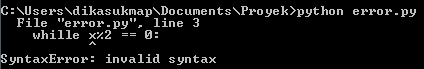
\includegraphics[width=0.85\textwidth]{figures/2/error.PNG}}
	\caption{Hasil menangkap pengecualian khusus}
	\label{fig:error}
\end{figure}
Kesalahan terdapat pada “whille”, perintah tersebut harusnya tidak menggunakan doubel l tetapi “while”.

\subsection{Kesalahan Logika}
Juga disebut kesalahan semantik, kesalahan logis menyebabkan program berperilaku tidak benar, tetapi mereka biasanya tidak crash program. Tidak seperti program dengan kesalahan sintaks, program dengan kesalahan logika dapat dijalankan, tetapi tidak beroperasi sebagaimana dimaksud. 

Pertimbangkan contoh kesalahan logis seperti pada listing \ref{lst:kesalahanlogika}:
\lstinputlisting[caption=Koding kesalahan logika, label={lst:kesalahanlogika}]{src/2/kesalahanlogika.py}

Contoh di atas harus menghitung rata-rata dari dua angka yang dimasukkan pengguna. Tetapi, karena urutan operasi dalam aritmatika (pembagian dievaluasi sebelum penambahan) program tidak akan memberikan jawaban yang benar seperti pada gambar \ref{fig:salahlogika}:
\begin{figure}[!htbp]
	\centerline{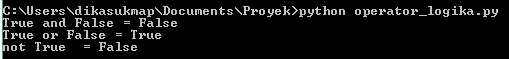
\includegraphics[width=0.85\textwidth]{figures/2/salahlogika.PNG}}
	\caption{Hasil program kesalahan logika}
	\label{fig:salahlogika}
\end{figure}

Untuk memperbaiki masalah ini, cukup menambahkan tanda kurung: z = (x + y) / 2
Ini adalah hasil yang benar seperti pada gambar \ref{fig:benarlogika}:
\begin{figure}[!htbp]
	\centerline{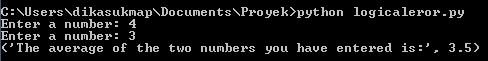
\includegraphics[width=0.85\textwidth]{figures/2/benarlogika.PNG}}
	\caption{Hasil setelah di benarkan}
	\label{fig:benarlogika}
\end{figure}

\section{Try to Except/pengecualian}
Python memiliki banyak exceptions bawaan yang memaksa program Anda untuk menghasilkan kesalahan ketika ada sesuatu yang salah di dalamnya. Ketika exceptions ini terjadi, itu menyebabkan proses saat ini berhenti dan meneruskannya ke proses panggilan sampai ditangani. Jika tidak ditangani, program ini akan macet.

Misalnya, jika fungsi A memanggil fungsi B yang pada gilirannya memanggil fungsi C dan pengecualian terjadi di fungsi C. Jika tidak ditangani dalam C, pengecualian beralih ke B dan kemudian ke A. Jika tidak pernah ditangani, pesan kesalahan dilemparkan dan program ini terhenti secara tiba-tiba.

\subsection{Menangkap Pengecualian dengan Python}
Dalam Python, pengecualian dapat ditangani menggunakan pernyataan coba. Operasi kritis yang dapat meningkatkan pengecualian ditempatkan di dalam klausa coba dan kode yang menangani pengecualian ditulis dalam kecuali klausa.

Contoh penggunaannya seperti pada listing \ref{lst:exception} :
\lstinputlisting[caption=Koding exception, label={lst:exception}]{src/2/exception.py}

Hasilnya seperti pada gambar \ref{fig:exception}:
\begin{figure}[!htbp]
	\centerline{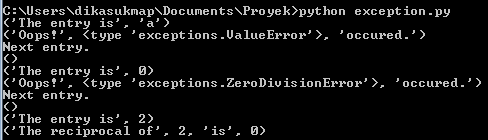
\includegraphics[width=0.85\textwidth]{figures/2/exception.PNG}}
	\caption{Hasil try to except}
	\label{fig:exception}
\end{figure}

Dalam program ini, anda harusi mengulang sampai pengguna memasukkan bilangan bulat yang memiliki timbal balik yang valid. Bagian yang dapat menyebabkan pengecualian ditempatkan di dalam blok try.

Jika tidak ada pengecualian terjadi, kecuali blok dilewati dan aliran normal berlanjut. Tetapi jika ada pengecualian terjadi, itu ditangkap oleh blok kecuali. System mencetak nama pengecualian menggunakan fungsi ex\_info () di dalam modul sys dan meminta pengguna untuk mencoba lagi. Anda dapat melihat bahwa nilai 'a' dan '1,3' menyebabkan ValueError dan '0' menyebabkan ZeroDivisionError.

\subsection{Menangkap Pengecualian Khusus dengan Python}
Dalam contoh di atas, pengecualian dalam klausa kecuali tidak disebutkan. Ini bukan praktik pemrograman yang baik karena akan menangkap semua pengecualian dan menangani setiap kasus dengan cara yang sama. Anda dapat menentukan pengecualian mana yang dikecualikan klausa kecuali.

Klausa coba dapat memiliki sejumlah kecuali klausa untuk menanganinya secara berbeda tetapi hanya satu yang akan dieksekusi jika terjadi pengecualian. Anda bisa menggunakan tupel nilai untuk menentukan beberapa pengecualian dalam klausa kecuali. 

Contoh penggunaannya seperti pada listing \ref{lst:specialexception} :
\lstinputlisting[caption=Koding special exception, label={lst:specialexception}]{src/2/specialexception.py}

\subsection{Meningkatkan Pengecualian}
Dalam pemrograman Python, pengecualian dimunculkan ketika kesalahan yang sesuai terjadi pada waktu berjalan, tetapi dapat dengan paksa menaikkannya menggunakan peningkatan kata kunci. Anda juga bisa memberikan nilai secara opsional pada pengecualian untuk mengklarifikasi mengapa pengecualian itu dinaikkan.

Contoh penggunaannya seperti pada listing \ref{lst:upexception} :
\lstinputlisting[caption=Koding meningkatkan pengecualian, label={lst:upexception}]{src/2/upexception.py}

\subsection{Try Finally}
Pernyataan coba dengan Python dapat memiliki klausa finally opsional. Klausa ini dieksekusi apa pun yang terjadi, dan umumnya digunakan untuk melepaskan sumber daya eksternal. Misalnya, anda dapat terhubung ke pusat data jarak jauh melalui jaringan atau bekerja dengan file atau bekerja dengan Graphical User Interface (GUI). 

Dalam semua keadaan ini, anda harus membersihkan sumber daya yang pernah digunakan, apakah itu berhasil atau tidak. Tindakan-tindakan ini (menutup file, GUI atau memutuskan sambungan dari jaringan) dilakukan pada klausa terakhir untuk menjamin eksekusi.

Contoh penggunaannya seperti pada listing \ref{lst:tryfinnaly} :
\lstinputlisting[caption=Koding try finnaly, label={lst:tryfinnaly}]{src/2/tryfinnaly.py}

Tipe konstruksi ini memastikan file ditutup bahkan jika pengecualian terjadi.



\bibliographystyle{IEEEtran} 
%\def\bibfont{\normalsize}
\bibliography{references}


%%%%%%%%%%%%%%%
%%  The default LaTeX Index
%%  Don't need to add any commands before \begin{document}
\printindex

%%%% Making an index
%% 
%% 1. Make index entries, don't leave any spaces so that they
%% will be sorted correctly.
%% 
%% \index{term}
%% \index{term!subterm}
%% \index{term!subterm!subsubterm}
%% 
%% 2. Run LaTeX several times to produce <filename>.idx
%% 
%% 3. On command line, type  makeindx <filename> which
%% will produce <filename>.ind 
%% 
%% 4. Type \printindex to make the index appear in your book.
%% 
%% 5. If you would like to edit <filename>.ind 
%% you may do so. See docs.pdf for more information.
%% 
%%%%%%%%%%%%%%%%%%%%%%%%%%%%%%

%%%%%%%%%%%%%% Making Multiple Indices %%%%%%%%%%%%%%%%
%% 1. 
%% \usepackage{multind}
%% \makeindex{book}
%% \makeindex{authors}
%% \begin{document}
%% 
%% 2.
%% % add index terms to your book, ie,
%% \index{book}{A term to go to the topic index}
%% \index{authors}{Put this author in the author index}
%% 
%% \index{book}{Cows}
%% \index{book}{Cows!Jersey}
%% \index{book}{Cows!Jersey!Brown}
%% 
%% \index{author}{Douglas Adams}
%% \index{author}{Boethius}
%% \index{author}{Mark Twain}
%% 
%% 3. On command line type 
%% makeindex topic 
%% makeindex authors
%% 
%% 4.
%% this is a Wiley command to make the indices print:
%% \multiprintindex{book}{Topic index}
%% \multiprintindex{authors}{Author index}

\end{document}

